\documentclass{subfile}

\begin{document}
  \section{Simulation Result}
  \subsection{Prediction on Termination on SIS and SIRS Epidemic Simulation Model}
  Since SIS and SIRS epidemic model takes a long time to terminate, and is not able to terminate within 100 iterations, prediction of termination is done using regression. The regression is based on 1 observation.

  \paragraph{Observation 1: }The decrease of peak infected value follows a concave up curve. In infected graphs of SIRS and SIS epidemic models, the peak decreases and when linked up, forms a concave up curve.

  \begin{center}
    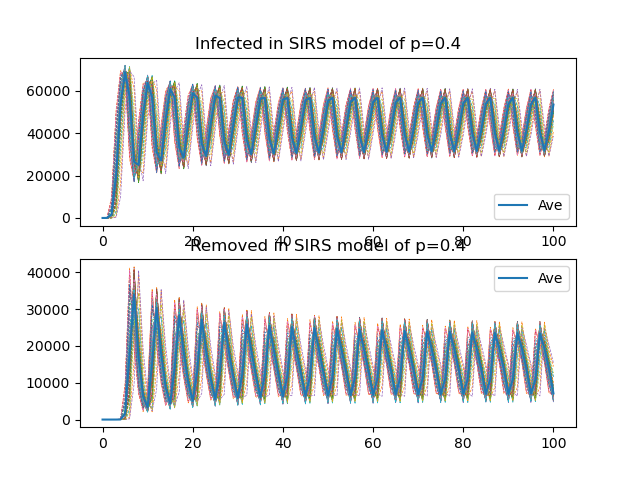
\includegraphics[scale=0.4]{sirsp04r1i3s3}
    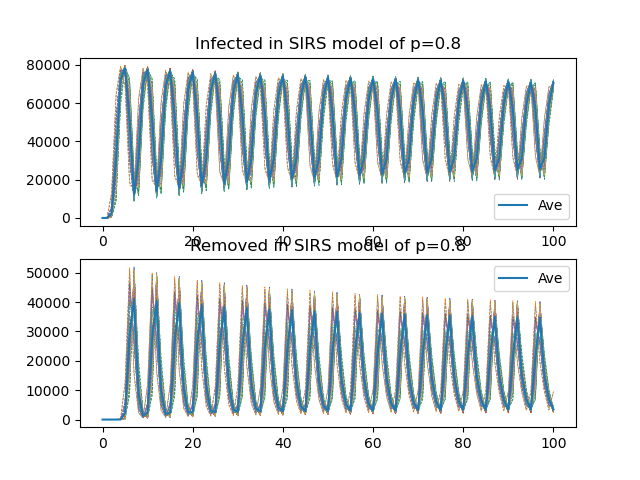
\includegraphics[scale=0.4]{sirsp08r1i3s3}
    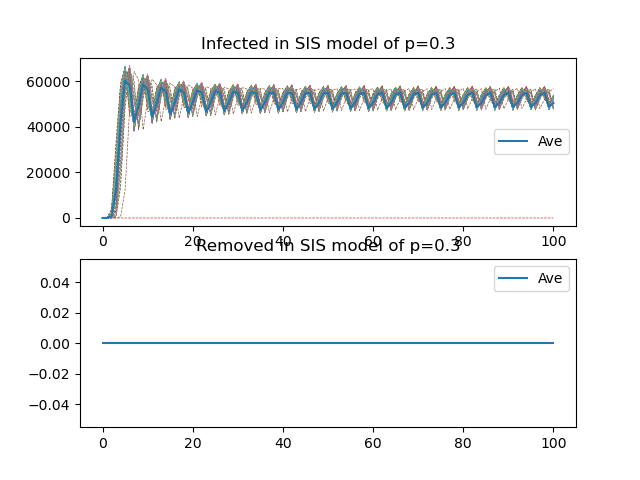
\includegraphics[scale=0.4]{sisp03r1i3s3}
    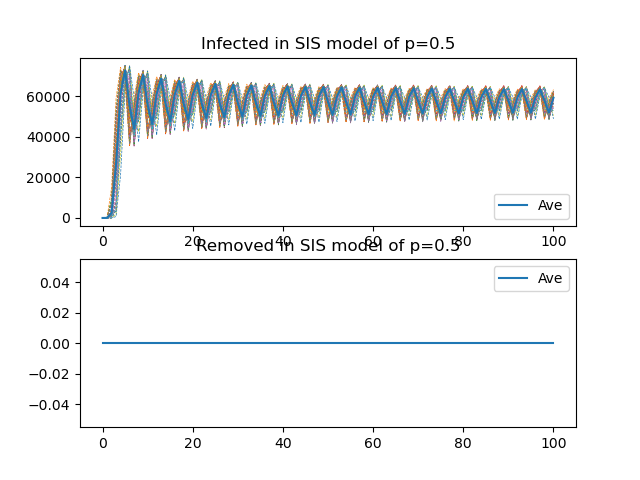
\includegraphics[scale=0.4]{sisp05r1i3s3}
    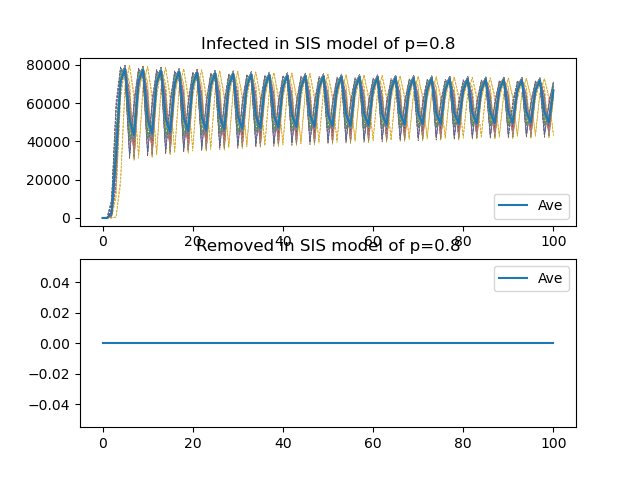
\includegraphics[scale=0.4]{sisp08r1i3s3}\\
  \end{center}
  \begin{figure}[h!]
  \centering
    \caption{Miniature graphs of SIRS and SIS Epidemic Model Simulation Result}
  \end{figure}

  Therefore, an educated geuss that the decay follows the logarithmic model \(y=w_1 log(x) + w_0\) is made. SIS and SIRS data are preprocessed by logarithmic transformation for linear regression for epidemic termination prediction.

  \begin{tabular}{cc}
    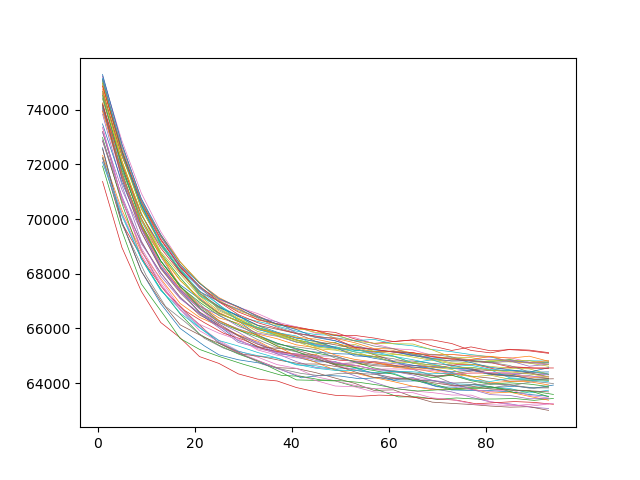
\includegraphics[scale=0.5]{SISp05chaos} & 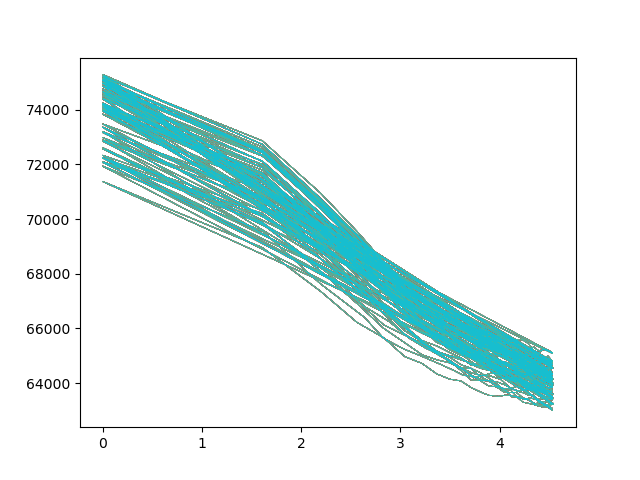
\includegraphics[scale=0.5]{logTrSISp05}\\
    Raw SIS peak value diagram & Log transform processed SIS peak value diagram\\
    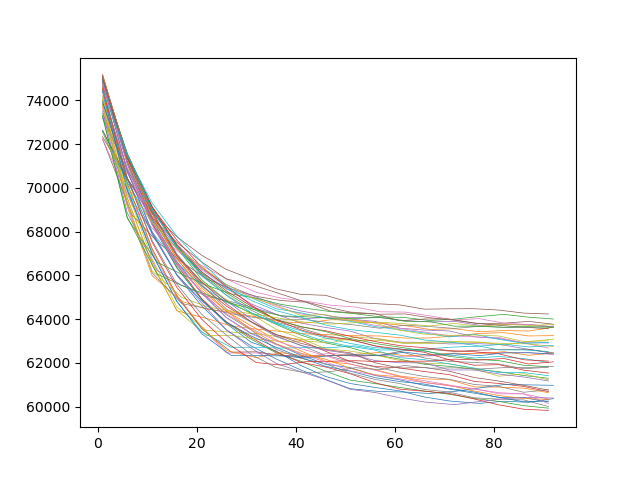
\includegraphics[scale=0.5]{SIRSp05chaos} & 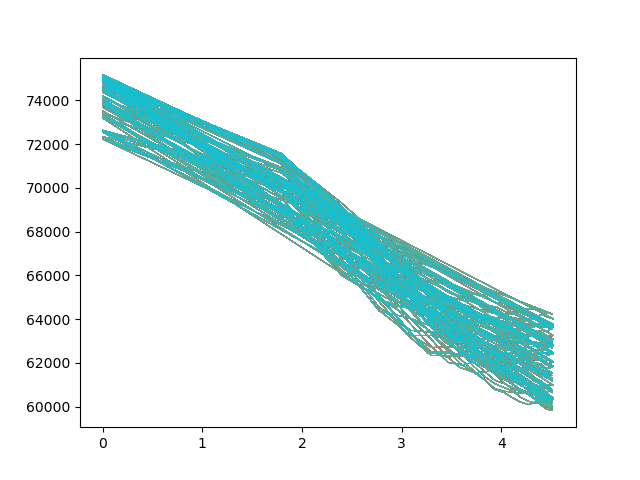
\includegraphics[scale=0.5]{logTrSIRSp05}\\
    Raw SIRS peak value diagram & Log transform processed SIRS peak value diagram\\
  \end{tabular}

  The result shows that the decay of peak values follows logarithmic model. Logarithmic transformation is applicable to some of the SIRS and SIS models.

  \subsection{Effect of Infection Probability}
  Model Simulation Parameters: \(i=3, r=1, s=3\)\\
  The following are the result from 100 simulations of each \(p\) levels of each epidemic model respectively.

  \subsubsection{SIR Simulation Result}
  {
  \begin{adjustbox}{max width=1.1\textwidth,center}
  \begin{tabular}{|l|l|l|l|l|l|l|l|l|l|l|}
    \hline
    SIR & p=0.1 & p=0.2 & p=0.3 & p=0.4 & p=0.5 & p=0.6 & p=0.7 & p=0.8 & p=0.9 & p=1.0\\
    \hline
    \makecell{Avg.\\Termination\\(\(t\)):} & 19.12 & 17.58 & 16.41 & 15.37 & 14.28 & 13.7 & 13.0 & 12.08 & 11.6 & 11.37\\
    \hline
    \makecell{Avg.\\Fraction of\\ Infected:} & 0.66472 & 0.85094 & 0.92685 & 0.96445 & 0.98348 & 0.99281 & 0.99729 & 0.99925 & 0.99991 & 1.0\\
    \hline
  \end{tabular}
  \end{adjustbox}}

  \subsubsection{SIRS Simulation Result}
  {
  \begin{adjustbox}{max width=1.2\textwidth,center}
  \begin{tabular}{|l|l|l|l|l|l|l|l|l|l|l|}
    \hline
    SIRS & p=0.1 & p=0.2 & p=0.3 & p=0.4 & p=0.5 & p=0.6 & p=0.7 & p=0.8 & p=0.9 & p=1.0\\
    \hline
    \makecell{Predicted\\Avg.\\Termination\\(\(t\))}: & \(5.9 + e^{12.378}\) & \(5.76 + e^{16.010}\) & \(5.26 + e^{23.423}\) & \(5.14 + e^{23.639}\) & \(5.08+e^{23.153}\) & \(4.9+e^{23.494}\) & \(4.78+e^{26.516}\) & \(4.82+e^{31.904}\) & \(4.74e^{40.203}\) & 12.0\footnotemark\\
    \hline
    \makecell{Avg. First\\Infection\\Peak:} & 5.9 & 5.76 & 5.26 & 5.14 & 5.08 & 4.9 & 4.78 & 4.82 & 4.74 & 4.74\\
    \hline
    \makecell{Avg. Wave\\Between Peak(\(t\):} & 5.0 & 5.0 & 5.0 & 5.0 & 5.0 & 5.0 & 5.0 & 5.0 & 5.0 & -\footnotemark\\
    \hline
    \makecell{Avg. Max\\Fraction\\of Infected:} & 0.50035 &  0.70016 & 0.79625 & 0.85564 & 0.90212 & 0.92747 & 0.94059 & 0.96067 & 0.96716 & 0.97088\\
    \hline
  \end{tabular}
  \end{adjustbox}}
  \footnotetext[4]{actual average termination is taken as when p=1.0, the SIRS model simulations succeeded in terminating}
  \footnotetext{SIRS p=1.0 does not persists in this social network}

  \subsubsection{SIS Simulation Result}
  {
  \small
  \begin{adjustbox}{max width=1.2\textwidth,center}
  \begin{tabular}{|l|l|l|l|l|l|l|l|l|l|l|}
    \hline
    SIS & p=0.1 & p=0.2 & p=0.3 & p=0.4 & p=0.5 & p=0.6 & p=0.7 & p=0.8 & p=0.9 & p=1.0\\
    \hline
    \makecell{Predicted\\Avg.\\Termination\\(\(t\)):} & \(6.0 + e^{6.5067}\) & \(5.66 + e^{35.1872}\) & \(5.32 + e^{31.7277}\) & \(5.18 + e^{30.3105}\) & \(5.06 + e^{29.5604}\) & \(4.96 + e^{29.5536}\) & \(4.76 + e^{30.7959}\) & \(4.92 + e^{37.5641}\) & \(4.68 + e^{49.4019}\) & -\footnotemark\\
    \hline
    \makecell{Avg. First\\Infection\\Peak:} & 6.0& 5.66& 5.32& 5.18& 5.06& 4.96& 4.76& 4.92& 4.68& 4.68\\
    \hline
    \makecell{Avg. Wave\\Between Peak(\(t\)):} & 4.0 & 4.0 & 4.0 & 4.0 & 4.0 & 4.0 & 4.0 & 4.0 & 4.0 & 4.0\\
    \hline
    \makecell{Avg. Max\\Fraction\\of Infected:} & 0.52313 & 0.68936 & 0.78111 & 0.85573 & 0.89919 & 0.92837 & 0.94482 & 0.95975 & 0.96489 & 0.97377\\
    \hline
  \end{tabular}
  \end{adjustbox}}
  \footnotetext{An increasing slope is observed in linear regression}

  \subsection{Effect of Length of Infection Period}
  Model Simulation Parameters: \(p=0.7, r=1, s=3\)\\
  The following are the result from 50 simulations of each \(i\) levels of each epidemic model respectively.

  \subsubsection{SIR Simulation Result}
  {\small
  \begin{adjustbox}{max width=1.2\textwidth,center}
  \begin{tabular}{|l|l|l|l|l|l|l|l|l|l|l|l|}
    \hline
    SIR & i=1& i=2& i=3& i=4& i=5& i=6& i=7& i=8& i=9& i=10& i=20\\
    \hline
    \makecell{Avg.\\Termination\\(\(t\)):} & 9.18&
11.44&
12.84&
14.14&
15.44&
16.74&
18.16&
19.34&
20.78&
21.88&
31.88\\
    \hline
    \makecell{Avg.\\Fraction of\\ Infected:}&0.94104&
0.98917&
0.99729&
0.99925&
0.99978&
0.99993&
0.99998&
0.99999&
1.0&
1.0&
1.0\\
    \hline
  \end{tabular}
  \end{adjustbox}}

  \subsubsection{SIRS Simulation Result}
  \begin{adjustbox}{max width=1.2\textwidth,center}
    \begin{tabular}{|l|l|l|l|l|l|l|l|l|l|l|l|}
      \hline
      SIRS & i=1 & i=2 & i=3 & i=4 & i=5 & i=6 & i=7 & i=8 & i=9 & i=10 & i=20\\
      \hline
      \makecell{Predicted\\Avg.\\Termination\\(\(t\))}\footnotemark: & \(3.68 + e^{4.6743}\) & \(4.16 + e^{19.4561}\) & \(4.87 + e^{26.8814}\) & \(901.4842\) & 1357.87 & 1913.31 & 3033.82 & 4475.72 & 7813.95 & 16386.95 & -\footnotemark\\
      \hline
      \makecell{Avg. First\\Infection\\Peak:} & 3.68 & 4.16 & 4.87 & 5.48 & 6.28 & 7.06 & 7.94 & 8.96 & 9.8 & 12.54 & 11.0\footnotemark\\
      \hline
      \makecell{Avg. Wave\\Between Peak(\(t\):} & 3.01 & 4.01 & 5.02 & 6.03 & 7.05 & 8.07 & 9.07 & 10.07 & 11.14 & 12.21 & \(\approx 23\)\footnotemark\\
      \hline
      \makecell{Avg. Max\\Fraction\\of Infected:} & 0.54819175& 0.83670018& 0.94382144& 0.98115787& 0.99390809& 0.99800506& 0.99927344& 0.9996624&  0.99984203& 0.9999243&  1.\\
      \hline
    \end{tabular}
  \end{adjustbox}
  \footnotetext[7]{Predicted Average Termination for \(i \geq 4\) used linear regression due to a positive \(R^2\) score in linear regression, not log regression and linear data ploted are not skewed and diverged}
  \footnotetext[8]{Non-negative slope detected in linear regression and fraction of infected reach 1.0 periodically}
  \footnotetext[9]{Infected fraction reach 1.0 at \(t=11\) in average}
  \footnotetext{Observation from figure of SIRS \(p=0.7,i=20,r=1,init\ infect=3\)}

  \subsubsection{SIS Simulation Result}
  \begin{adjustbox}{max width=1.2\textwidth,center}
    \begin{tabular}{|l|l|l|l|l|l|l|l|l|l|l|l|}
      \hline
      SIS & i=1 & i=2 & i=3 & i=4 & i=5 & i=6 & i=7 & i=8 & i=9 & i=10 & i=20\\
      \hline
      \makecell{Predicted\\Avg.\\Termination\\(\(t\))}\footnotemark: & \(3.62 + e^{4.0091}\) & \(4.26 + e^{24.959}\) & \(4.8 + e^{30.138}\) & \(5.54 + e^{39.511}\) & 1602.9 & 2497.2 & 3664.3 & 5512.0 & 16532.27 & 16386.95 & -\footnotemark\\
      \hline
      \makecell{Avg. First\\Infection\\Peak:} & 3.62& 4.26& 4.8& 5.54& 6.18& 7.0& 7.94& 8.66& 9.54& 12.18 & 11.0\footnotemark\\
      \hline
      \makecell{Avg. Wave\\Between Peak(\(t\):} & 2.0055 & 3.0026 & 4.0026 & 5.0111 & 6.0280 & 7.0338 & 8.0364 & 9.1039 & 10.090 & 11.163 & \(\approx21\)\footnotemark\\
      \hline
      \makecell{Avg. Max\\Fraction\\of Infected:} & 0.56421& 0.83312& 0.94710& 0.98251& 0.99392& 0.99800&
 0.99928& 0.99971&  0.99985& 0.99992& 1.0000\\
      \hline
    \end{tabular}
  \end{adjustbox}
  \footnotetext[11]{For \(i\geq 5\), the peak:time graph approaches linear}
  \footnotetext[12]{Non-negative slope detected in linear regression of data and fraction of infected reach 1.0 periodically}
  \footnotetext[13]{Infected fraction reach 1.0 at \(t=11\) in average}
  \footnotetext{Observation from figure of SIS \(p=0.7,i=20,r=1,init\ infect=3\)}

  \subsection{Effect of Numbers of Initial Infected}
  Model Simulation Parameters: \(p=0.7, r=1, i=3\)\\
  The following are the result from 50 simulations of each \(s\) levels of each epidemic model respectively.

  \subsubsection{SIR Simulation Result}
  {
  \begin{adjustbox}{max width=1.1\textwidth,center}
  \begin{tabular}{|l|l|l|l|l|l|l|l|l|l|l|}
    \hline
    SIR & s=1 & s=2 & s=3 & s=4 & s=5 & s=6 & s=7 & s=8 & s=9 & s=10\\
    \hline
    \makecell{Avg.\\Termination\\(\(t\)):} & 13.48 & 13.06 & 12.84 & 12.58 & 12.64 & 12.64 & 12.42 & 12.5 & 12.5 & 12.32\\
    \hline
    \makecell{Avg.\\Fraction of\\ Infected:}& 0.99727 &
0.99731 &
0.99729 &
0.99730 &
0.99732 &
0.99729 &
0.99733 &
0.99726 &
0.99735 &
0.99731 \\
    \hline
  \end{tabular}
  \end{adjustbox}}

  \subsubsection{SIRS Simulation Result}
  {
  \begin{adjustbox}{max width=1.1\textwidth,center}
    \begin{tabular}{|l|l|l|l|l|l|l|l|l|l|l|}
      \hline
      SIRS & s=1 & s=2 & s=3 & s=4 & s=5 & s=6 & s=7 & s=8 & s=9 & s=10\\
      \hline
      \makecell{Predicted\\Avg.\\Termination\\(\(t\))}: & \(5.3 + e^{25.788}\) & \(5.04 + e^{24.616}\) & \(4.86 + e^{26.881}\) & \(4.76 + e^{26.255}\) & \(4.7 + e^{26.806}\) & \(4.7 + e^{27.585}\) & \(4.52 + e^{29.612}\) & \(4.36 + e^{28.599}\) & \(4.44 + e^{27.806}\) & \(4.34 + e^{28.121}\)\\
      \hline
      \makecell{Avg. First\\Infection\\Peak:}& 5.3& 5.04& 4.86& 4.76& 4.7& 4.7& 4.52& 4.36& 4.44& 4.34\\
      \hline
      \makecell{Avg. Wave\\Between Peak(\(t\):}& 5.0267& 5.0189& 5.0211& 5.0178& 5.0211& 5.0178& 5.0267& 5.0356& 5.03& 5.0355\\
      \hline
      \makecell{Avg. Max\\Fraction\\of Infected:}& 0.946& 0.94776& 0.94382& 0.94591& 0.94373& 0.94148& 0.93761& 0.93893& 0.94044& 0.93847\\
      \hline
    \end{tabular}
  \end{adjustbox}}

  \subsubsection{SIS Simulation Result}
  {
  \begin{adjustbox}{max width=1.1\textwidth,center}
    \begin{tabular}{|l|l|l|l|l|l|l|l|l|l|l|}
      \hline
      SIS & s=1 & s=2 & s=3 & s=4 & s=5 & s=6 & s=7 & s=8 & s=9 & s=10\\
      \hline
      \makecell{Predicted\\Avg.\\Termination\\(\(t\))}: & \(5.12 + e^{18.581}\) & \(5.0+ e^{30.855}\) & \(4.8+ e^{30.138}\) & \(4.84 + e^{31.349}\) & \(4.66 + e^{30.956}\) & \(4.54 + e^{30.303}\) & \(4.42 + e^{30.479}\) & \(4.48 + e^{31.245}\) & \(4.52 + e^{31.340}\) & \(4.4 + e^{31.886}\)\\
      \hline
      \makecell{Avg. First\\Infection\\Peak:}& 5.12& 5.0& 4.8& 4.84& 4.66& 4.54& 4.42& 4.48& 4.52& 4.4\\
      \hline
      \makecell{Avg. Wave\\Between Peak(\(t\):}& 4.0061& 4.0052& 4.0026& 4.0026& 4.007& 4.0052& 4.0061& 4.007& 4.0052& 4.007\\
      \hline
      \makecell{Avg. Max\\Fraction\\of Infected:}& 0.94478& 0.94469& 0.9471& 0.94224& 0.94001& 0.94015& 0.94142& 0.94017& 0.93989& 0.93943\\
      \hline
    \end{tabular}
  \end{adjustbox}}

  \subsection{Effect of Length of Removed Period}
  Model Simulation Parameters: \(p=0.7, i=3, s=3\)\\
  The following are the result from 50 simulations of each \(r\) levels of each epidemic model respectively.\\
  Only SIRS model will be tested as SIS model have no removed state and SIR model will not convert back to susceptible state after removed.

  \subsubsection{SIRS Simulation Result}
  \begin{adjustbox}{max width=1.2\textwidth,center}
    \begin{tabular}{|l|l|l|l|l|l|l|l|l|l|l|}
      \hline
      SIRS & r=1 & r=2 & r=3 & r=4 & r=5 & r=6 & r=7 & r=8 & r=9& r=10\\
      \hline
      \makecell{Predicted\\Avg.\\Termination\\(\(t\)):}\\
      \hline
      \makecell{Avg. First\\Infection\\Peak:}\\
      \hline
      \makecell{Avg. Wave\\Between Peak(\(t\)):}\\
      \hline
      \makecell{Avg. Max\\Fraction\\of Infected:}\\
      \hline
    \end{tabular}
  \end{adjustbox}

  \subsection{Effect of Network Structure on Epidemic Models}

\end{document}
